 % Theory of elasticity and failure
 \chapter{Elasticity and failure}
 To have a framework upon which to discuss failure and fracture in methane hydrates, we need some theory of elasticity and failure of elastic materials. This will also be needed in order to be explicit about how stresses and strains are imposed on model systems.

 \section{Linear elasticity}
Since I will deal with possibly anisotropic matrials, I start with the general tensor form of Hooke's law, and then provide the simplifications resulting from an isotropic material.
The generalized Hooke's law	is:
\begin{equation}
	\sigma_{ij} = c_{ijkl}\epsilon_{kl}
\end{equation}
This law relates the Cauchy stress tensor $\sigma_{ij}$ to the strain tensor $\epsilon_{kl}$ in a linearly elastic material. All material properties are contained in the stiffnes tensor $c_{ijkl}$.
In this form, Hooke's law basically states that ``each component of the cauchy stress tensor depends linearly on all components of the strain tensor''. 

Hooke's law contains two tensors of rank 2 with 9 components each, and one tensor of rank 4 with 81 componens. Luckily, there are symmetries to be exploited. First, the Cauchy stress tensor is symmetric, which leads to $c_{ijkl} = c_{jikl}$. Second, the strain tensor is symmetric, so $c_{ijkl} = c_{ijlk}$. This means we are left with 6 independent combination of each of $ij$ and $kl$, and a total of 36 components. 

Using the rank reduction method of Voigt, the stess and strain matrices can be written as vectors:
\begin{equation}
	\uuline{\sigma} = 
	\begin{pmatrix}
	\sigma_{11} & \sigma_{12} & \sigma_{13} \\
	\sigma_{21} & \sigma_{22} & \sigma_{23} \\
	\sigma_{31} & \sigma_{32} & \sigma_{33} \\ 
	\end{pmatrix}
	\to 
	\vec{\sigma} = 
	\begin{pmatrix}
	\sigma_{11} \\ \sigma_{22} \\ \sigma_{33} \\ \sigma_{23} \\ \sigma_{13} \\ \sigma_{12}
	\end{pmatrix}
	\equiv
	\begin{pmatrix}
	\sigma_{1} \\ \sigma_{2} \\ \sigma_{3} \\ \sigma_{4} \\ \sigma_{5} \\ \sigma_{6}
	\end{pmatrix}
\end{equation}

\begin{equation}
	\uuline{\epsilon} = 
	\begin{pmatrix}
	\epsilon_{11} & \epsilon_{12} & \epsilon_{13} \\
	\epsilon_{21} & \epsilon_{22} & \epsilon_{23} \\
	\epsilon_{31} & \epsilon_{32} & \epsilon_{33} \\ 
	\end{pmatrix}
	\to 
	\vec{\epsilon} = 
	\begin{pmatrix}
	\epsilon_{11} \\ \epsilon_{22} \\ \epsilon_{33} \\ 2\epsilon_{23} \\ 2\epsilon_{13} \\ 2\epsilon_{12}
	\end{pmatrix}
	\equiv
	\begin{pmatrix}
	\epsilon_{1} \\ \epsilon_{2} \\ \epsilon_{3} \\ \epsilon_{4} \\ \epsilon_{5} \\ \epsilon_{6}
	\end{pmatrix}
\end{equation}

For the same reasons, the stiffness tensor can be recuced to rank 2 (I choose not to write out the complete stiffness tensor, only the reduced one):
\begin{equation}
	\vec{C} =
	\begin{pmatrix}
	C_{11} & C_{12} & C_{13} & C_{14} & C_{15} & C_{16} \\
	C_{21} & C_{22} & C_{23} & C_{24} & C_{25} & C_{26} \\
	C_{31} & C_{31} & C_{33} & C_{34} & C_{35} & C_{36} \\
	C_{41} & C_{42} & C_{43} & C_{44} & C_{45} & C_{46} \\
	C_{51} & C_{52} & C_{53} & C_{54} & C_{55} & C_{56} \\
	C_{61} & C_{62} & C_{63} & C_{64} & C_{65} & C_{66}
	\end{pmatrix}
\end{equation}
Hooke's law can now be written as a matrix equation:
\begin{equation}
	\vec{\sigma} = \vec{C}\vec{\epsilon}
\end{equation}

It actually turns out that the stiffness matrix is symmetric, because stress and strain are work-conjugates:
\begin{equation}
	\sigma_i = \frac{\partial u}{\partial \epsilon_i}
\end{equation}
Where $u$ is the energy density associated with the stress-strain configuration.
Insering this into Hooke's law gives:
\begin{equation}
	C_{ij}=\frac{\partial^2 u}{\partial \epsilon_i \partial \epsilon_j} = \frac{1}{V} \frac{\partial^2 U}{\partial \epsilon_i \partial \epsilon_j} 
\end{equation}
This latter relation is useful for estimating the stiffness matrix from molecular simulation, as strains are easy to impose, and energy is trivial to measure.

\subsection{Isotropic materials}
Isotropic materials can be described by two parameters: Youngs modulus $E$ and poissons ratio $\nu$. The nature of the definition of these quantities leads to the stiffness matrix for isotropic materials:
\begin{equation}
	\vec{C} = 
   	\frac{E}{(1+\nu)(1-2\nu)}
   	\begin{pmatrix}
		1-\nu & \nu & \nu & 0 & 0 & 0 \\
		\nu & 1-\nu & \nu & 0 & 0 & 0 \\
		   \nu & \nu & 1-\nu & 0 & 0 & 0 \\
		   0 & 0 & 0 & (1-2\nu)/2 & 0 & 0 \\
		   0 & 0 & 0 & 0 & (1-2\nu)/2 & 0 \\
		   0 & 0 & 0 & 0 & 0 & (1-2\nu)/2
	\end{pmatrix}
\end{equation}

\subsection{Plane strain and plane stress}
Plane strain and plane stress are conditions where a three-dimensional elastic problem can be analyzed as two-dimensional ones. The formal definitions of plane strain and plane stress are given in equations \ref{eq:plane_strain} and \ref{eq:plane_stress}, respectively.

\begin{equation}
\uuline \epsilon = 
\begin{pmatrix}
	\epsilon_{11} & \epsilon_{12} & 0 \\
	\epsilon_{21} & \epsilon_{22} & 0 \\
	0 & 0 & 0
\end{pmatrix}
\label{eq:plane_strain}
\end{equation}

\begin{equation}
\uuline \sigma = 
\begin{pmatrix}
	\sigma_{11} & \sigma_{12} & 0 \\
	\sigma_{21} & \sigma_{22} & 0 \\
	0 & 0 & 0
\end{pmatrix}
\label{eq:plane_stress}
\end{equation}

For plane strain, we allow a nonzero stress component $\sigma_{33}$, and likewise, for plane stress we allow a nonzero strain component $\epsilon_{33}$. However, these components can only be results of the analysis, they shall not enter the analysis. 


\section{Simple fracture mechanics}
In linear elastic fracture mechanics (LEFM), there are essentially two quantities that govern failure: The stress intensity factor $K$, and the energy release rate $G$. For linear elastic materials, these are uniquely related.

\subsection{Brittle and ductile materials}
In materials science, it is common to distinguish between brittle and ductile materials. According to Wikipedia, a material i brittle if it ``breaks without significant strain'', whereas ductility is ``a solid material's ability to deform under tensile stress''. Deformation in this context is plastic. It is actually hard to come along a more satisfying definition -- ductility and brittleness seems to be the kind of knowledge that everyone in the field have, but no one writes down as an equation. Throughout this thesis, I will use the term brittle -- by which i will be meaning ideally brittle -- about failure where the material acts completely elastic when subected to strain, until it suddenly breaks over essentialy no change in the strain.

\begin{figure}
\centering
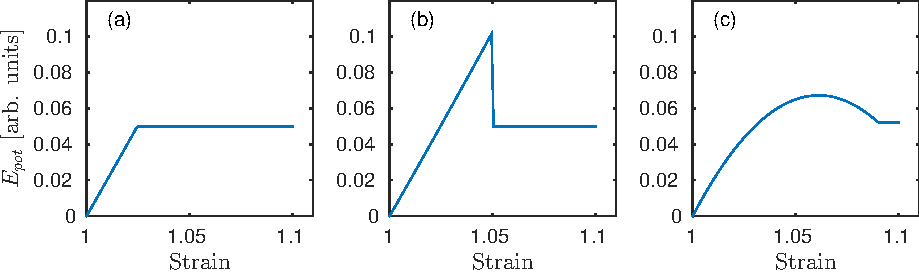
\includegraphics[width=\textwidth]{../figures/thesis/idealized_fracture_e_pot.pdf}
\caption{Potential energy as a function of applied strain for systems held at a constant temperature. The figure shows three idealized examples of failure. (a) and (b) are brittle, (c) is ductile. In (a), the system reaches a stress state where $G_c = 2\gamma_s$ and breaks. No energy is lost to plastic deformation or heat. In (b), the system breaks at $G_c > 2\gamma_s$ and energy is lost to heat, but not to plastic deformation. In (c), the system is continously deforming plastically through the straining process -- the material is very ductile. Note that it is not possible to see the amount of energy lost to plastic deformation from (c). The plateau in all figures represents a state where a crack propagated through the whole system -- the system is divided into two parts -- so additional straining does not contribute potential energy. }
\end{figure}

\subsection{Modes of loading}
It is common to distinguish between three different forms of crack loading: I =`opening', II = `sliding', III = `tearing'. 

\begin{figure}
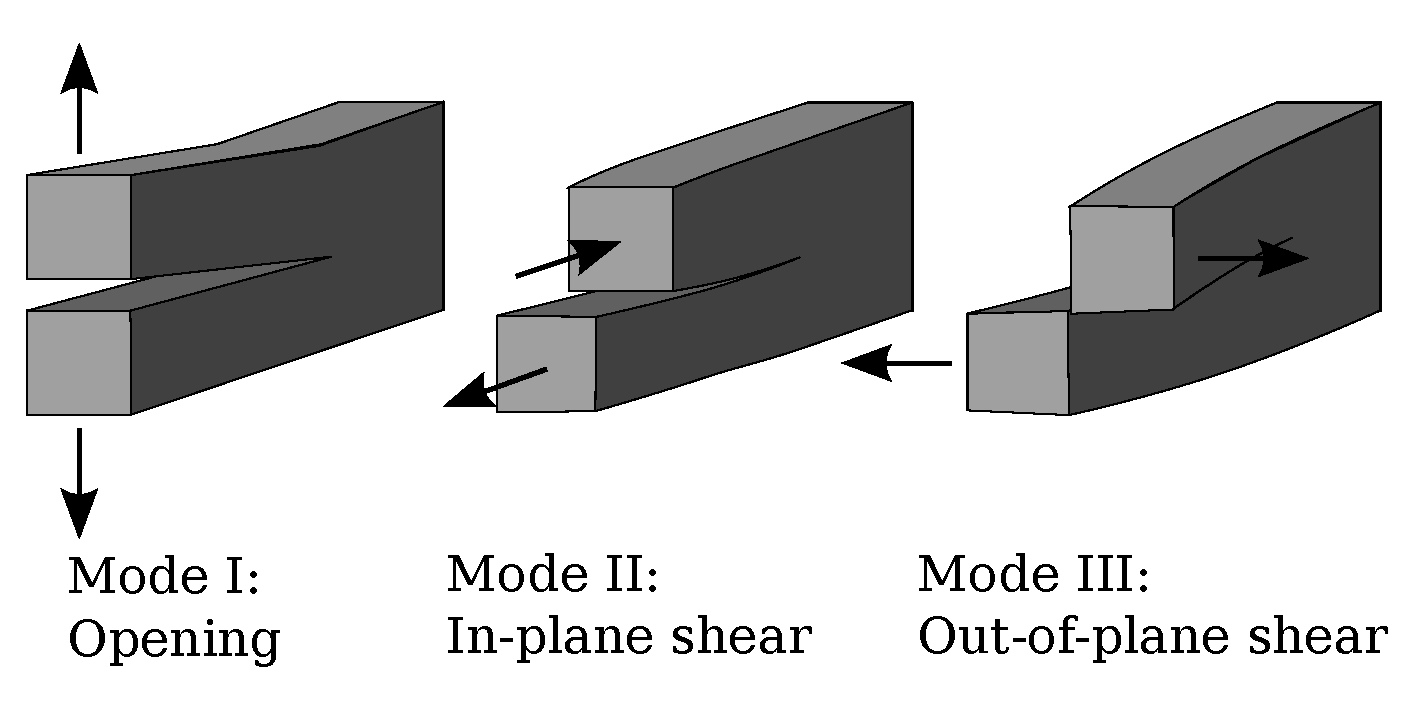
\includegraphics[width=\textwidth]{../figures/thesis/Fracture_modes_v2.pdf}
\caption{Three modes of crack separation. (``Fracture modes v2'' by Twisp - This vector image was created with Inkscape. Licensed under Public Domain via Wikimedia Commons)}
\end{figure}

\subsection{Failure criteria.}
As is many fields, the first recorded studies the ones of Leonardo da Vinci. Leonardo discovered that short iron wires are stronger than long steel wires. A common interpretation is that random flaws make the iron wires weaker at some points, and that a longer wire has a larger probability of a weak spot than a long one. A major goal of fracture mechanics is to be able to predict the failure of structures -- what is the pressure required to break a sample of a material? The first somewhat successful attempt to predict failure was the efforts of Inglis. He introduced the concept of stress concentration at a crack tip. Specifically, he found that for an elliptical crack on an infinite sheet, the local stress at the crack tip as a function of the faraway tensile stress was:

\begin{equation}
	\sigma_{\text{cracktip}} = 2\sigma_{\text{faraway}}\sqrt{\frac{a}{\rho}}
	\label{eq:stress_consentration}
\end{equation}
Where $a$ is the length of the major axis of the ellipsis, and $\rho$ is the radius of curvature of the ellipsis close to the crack tip. The local critical stress level is the stress needed to break atomic bonds \cite[p. 27]{Anderson2005}:

\begin{equation}
	\sigma_c = \sqrt{\frac{E\gamma_s}{x_0}}
	\label{eq:critical_local}
\end{equation}
Where $x_0$ is the typical distance between atoms. Now setting the cracktip stress from equation \ref{eq:stress_consentration} equal to the critical local stress from equation \ref{eq:critical_local}, and assuming that the radius of curvature is equal to the distance between atoms, we get an expression for the critical faraway stress level:
\begin{equation}
	\sigma_f = \sqrt{\frac{E\gamma_s}{4a}}
	\label{eq:inglis_formula}
\end{equation}
Which is the Inglis formula for the fracture stress on a large sheet with a crack of width $2a$.

In 1920, Griffith improved on the flaw-approach, but instead of building a theory from the atomic level, he assumed the following: A crack will propagate from a flaw if the strain energy released during crack growth is higher than the corresponging surface energy from crack growth. This works well for ideally brittle materials. The formula for critical faraway stress with Griffiths theory is:
\begin{equation}
	\sigma_f = \sqrt{\frac{2E\gamma_s}{\pi a}}
\end{equation}
Which is the Griffith formula for the fracture stress on a large sheet with a frack of width $2a$. For reference, I also include the formula for the fracture stress of a penny-shaped crack subjected to remote tensile stress:
\begin{equation}
	\sigma_f = \sqrt{\frac{\pi E \gamma_s }{2(1-\nu^2)a}}
\end{equation}
 
 For a sheet of finite width, the fracture stress is slightly lower, since the crack actually weakens the materal (the cross sectional area bearing the stress is shrinking). The exact expression for a sheet of width $2W$ is:

 \begin{equation}
 	\sigma_f = \sqrt{\frac{2\gamma_s E}{2W\tan\left( \frac{\pi a}{2W}\right)}}
 	\label{eq:griffith_finite_sheet}
 \end{equation}

 Irwin refined Griffiths approach, and introduced the \emph{energy release rate}, $\mathcal{G}$. The energy release rate is a property of the elastic state of a linearly elastic material. According to Irwin, a crack will propagate when $\mathcal{G}$ becomes larger than a material-specific value $\mathcal{G}_c$ -- the \emph{critical} energy release rate. For a crack of width $2a$ on an infinite plate subjected to tensile stress, the energy release rate is:

\begin{equation}
	\mathcal{G} = \frac{\pi \sigma^2 a}{E}
\end{equation}

This is a purely a relation concerning how a linear elastic material distributes energy during crack opening. This means that the longer the crack, the more energy is available for crack opening at a given stress.

The critial value can be measured experimentally using a sample with an artificial flaw whose length is known and measure the yield pressure. 

For linear elastic materials, the energy release rate is equivalent to another measure, the \emph{stress intensity factor}, $K$. The stress intensity factor is a constant of proportionality between the applied stress on a crack and the stress distribution around the crack tip. For mode I loading it is:
\begin{equation}
	\lim_{r \to 0} \sigma_{ij}^I = \frac{K_I}{\sqrt{2\pi r}} f_{ij}(\theta)
\end{equation}
Where $r$ is the distance from the crack tip and $\theta$ is the angle from the crack axis. Both the energy release rate and the stress intensity factor concern the distribution of a remote stress, but the stress intensity factor says how the stress is distributed near the crack tip, whereas the energy release rate says how much mechanical energy will released if the new crack surface opens. @FinishSection


\subsection{Stress intensity factors in anisotropic materials}
Simple fracture theory assumes that one only need one parameter to describe the fracture properties of a material, the critical stress intensity factor under tensile loading -- the fracture toughness. I will need a procedure to obtain that from molecular dynamics simulations. Having obtained the fracture area and the energy release rate, I can use the generalized irwin formula @citation to calculate the stress intensity factor. 

\begin{equation}
	G = \pi \vec{K}^T [\vec{H}] \vec{K} 
\end{equation}

Where $\vec{H}$ is a matrix that depends on the elastic properties of the material. This expression is valid for a plane crack propagating in two opposite directions with symmetric load with respect to the two directions of crack propagation.
To find the stress intensity factor for mode I loading, I only need to ensure a pure mode I loading situation, and obtain the element $H_{11}$. This matix element was worked out by \cite{Laubie2014}, and is:

\begin{equation}
	H_{11} = \frac{1}{2\pi} \sqrt{\frac{C_{11}}{C_{11}C_{33}-C^2_{13}}\left( \frac{1}{C_{44}} + \frac{2}{C_{13} + \sqrt{C_{11} C_{33}}}\right)}
\end{equation}

The stress intensity factor for mode I loading is the standard for fracture toughness measures. @ElegantClosingSentence

For the special case of isotropic materials under mode I loading, we recover a more familiar expression, Irwins formula for plane strains:

\begin{equation}
	K_c = \sqrt{\frac{EG_c}{1-\nu^2}}
	\label{eq:energy_release_to_stress_intensity_isotropic}
\end{equation}

\section{Stress consentrations around an elliptical hole}
There are several analytical solutions for stress concentrations for isotropic materials with failures of specific geometries. A particularly interesting solution for my purposes is the stress concentration near the crack tip of an elliptic crack in an infinitely large sheet of linearly elastic and isotropic material \cite{Anderson2005}. I give the equations for a crack along the y-axis with a stress applied along the x-axis.

\begin{align}
	\sigma_{xx} & =  \frac{K_I}{\sqrt{2\pi r}} \cos\left(\frac{\theta}{2}\right) \left[ 1+\sin\left(\frac{\theta}{2} \right)\sin\left( \frac{3\theta}{2}\right)\right]\\
	\sigma_{yy} & =  \frac{K_I}{\sqrt{2\pi r}} \cos\left(\frac{\theta}{2}\right) \left[ 1-\sin\left(\frac{\theta}{2} \right)\sin\left( \frac{3\theta}{2}\right)\right]\\	
	\tau_{xy} & =  \frac{K_I}{\sqrt{2\pi r}} \cos\left(\frac{\theta}{2}\right)\sin\left(\frac{\theta}{2} \right)\cos\left( \frac{3\theta}{2}\right)
\end{align}

\begin{figure}
\centering
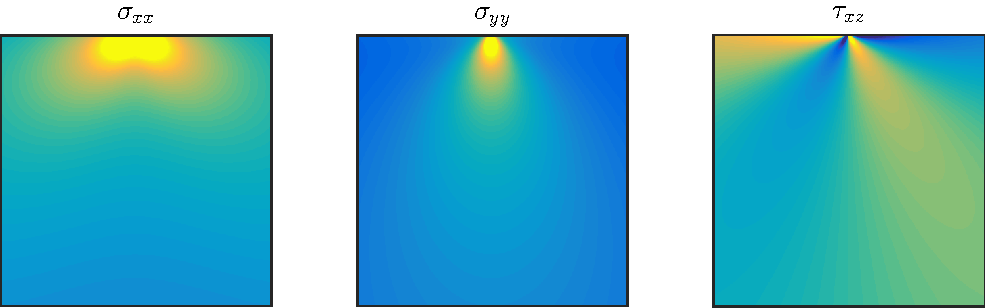
\includegraphics[width=\textwidth]{../figures/thesis/analytic_stress.pdf}
\caption{Near crack-tip stress for a plane crack along the y-axis. The crack tip is located at the top center of each plot.}
\label{fig:analytic_stress}
\end{figure}

